%        File: dual_averaging_relaxed_clustering.tex
%     Created: Wed May 21 12:00 PM 2014 C
% Last Change: Wed May 21 12:00 PM 2014 C
%
\documentclass[a4paper]{article}

\usepackage[utf8]{inputenc}
\usepackage[french]{babel}
\usepackage[left=4cm, right=4cm, top=4cm, bottom=4cm]{geometry}

\usepackage{amsmath}
\usepackage{amsfonts}

\usepackage{algpseudocode}
\usepackage{algorithm}
\DeclareMathOperator*{\argmin}{arg\,min}

\usepackage{cite}
\usepackage{graphicx}

\title{Optimisation distribuée pour la résolution d'un problème
    de \emph{clustering}}
\author{Igor Colin}
\date{\today}

\begin{document}

\maketitle

\section{Description du problème}
\label{sec:description_probleme}

\subsection{Problème initial}
\label{sub:probleme_initial}

Soit $\mathcal{X}$ un espace de dimension finie et soit
$(X_i)_{1 \leq i \leq n}$ $n$ points dans $\mathcal{X}$. Pour $K > 0$,
on cherche à résoudre le problème de clustering suivant
\cite{clemenccon2014statistical}:
\begin{equation}
    \label{eq:clustering_initial}
    \min_{P \in \mathcal{P}_K} f(P) =
    \frac{1}{n^2} \sum_{1 \leq i,j \leq n} D(X_i, X_j) \Phi_P(i, j)
\end{equation}

où $\mathcal{P}_K$ est l'ensemble des partitions de taille $K$ de
$\{1,\ldots,n\}$, $D$ est une mesure de dissimilarité entre les éléments de
$\mathcal{X}$ et $\Phi_P$ est définie pour tout $P \in \mathcal{P}_K$ par:
\[
    \Phi_P : \left\{
        \begin{array}{r c l}
            \left\{ 1,\ldots,n \right\}^2 & \rightarrow & \left\{ 0, 1 \right\}\\
            (i, j) & \mapsto &
            \begin{cases}
                1 & \text{si } i \text{ et } j \text{ sont dans le même \emph{cluster}} \\
                0 & \text{sinon}
            \end{cases}
        \end{array}
    \right.
\]
La mesure de dissimilarité $D$ doit vérifier les propriétés suivantes :
\begin{description}
    \item[Symétrie] : Pour $(x, x') \in \mathcal{X}^2$, $D(x, x') = D(x', x)$
    \item[Séparation] : Pour $(x, x') \in \mathcal{X}^2$, $D(x, x') = 0$
        si et seulement si $x = x'$
\end{description}

On remarque qu'en définissant, pour $1 \leq i \leq n$,
\[
    f_i : \left\{
        \begin{array}{r c l}
            \mathcal{P}_K & \rightarrow & \mathbb{R}_+ \\
            P & \mapsto & \frac{1}{n} \sum_{j = 1}^n D(X_i, X_j) \Phi_P(i, j)
        \end{array}
    \right.
\]
on peut réécrire le problème~(\ref{eq:clustering_initial}) sous la forme:
\begin{equation}
    \label{eq:clustering_distribue}
    \min_{P \in \mathcal{P}_K} \frac{1}{n} \sum_{i = 1}^n f_i(P)
\end{equation}
Dans cette formulation, nous avons seulement décomposé la fonction objectif
$f$ en $n$ fonctions objectifs partielles.

\subsection{Contraintes supplémentaires}
\label{sub:contraintes_supplementaires}

On souhaite résoudre le problème de \emph{clustering} précédent de
manière distribuée.
On considère pour cela un graphe non-orienté $G = (V, E)$, où
$V = \left\{ 1, \ldots, n \right\}$. Chaque sommet $i \in V$ du graphe
représente un agent, capable de calculer uniquement les valeurs de $f_i$
sur $\mathcal{P}_K$. On considère également que les différents agents sont
capables de communiquer (i.e.\ donner la valeur de leur fonction objectif
partielle en un point), avec leur voisinage. C'est-à-dire que deux agents
$(i, j) \in V^2$ pourront communiquer entre eux si et seulement si
$(i, j) \in E$.

\section{Résolution du problème}
\label{sec:resolution_du_probleme}

\subsection{Algorithme de moyennage de dual distribué}
\label{sub:dual_averaging}


Les méthodes d'optimisation ou de classification distribuée sont nombreuses et
variées. Afin de pouvoir facilement adapter la méthode à notre problème, on se
penchera sur des techniques génériques, demandant peu d'hypothèses sur la
structure du problème. On souhaite également utiliser des algorithmes
possédant de bonnes garanties théoriques concernant leur vitesse de convergence
ainsi que leur précision. Pour ces raisons, nous nous concentrerons par la
suite sur l'algorithme de moyennage de dual distribué \cite{duchi2012dual,
nesterov2009primal, xiao2010dual}.

Cette méthode est adaptée de la méthode de moyennage de dual visant à résoudre
le problème d'optimisation suivant:
\begin{equation}
    \label{eq:optimisation_convexe}
    \min_{x \in \mathcal{X}} f(x)
\end{equation}
où $\mathcal{X} \subset \mathbb{R}^d$ est un fermé convexe et $f$ est une
fonction convexe, sous-différentiable sur $\mathcal{X}$ et $L$-lipschitzienne
pour un certain $L > 0$. Le moyenne de dual repose fortement sur l'utilisation
d'un opérateur proximal $\psi : \mathcal{X} \rightarrow \mathbb{R}$, fortement
convexe sur $\mathcal{X}$ par rapport à une certaine norme $N$. Le choix du
couple $(\psi, N)$ s'effectuera en fonction du problème considéré. Par exemple,
si $\mathcal{X}$ est le simplexe de $\mathbb{R}^d$, on aura tendance à choisir
la fonction d'entropie pour $\psi$ et la norme-$1$ pour $N$. L'idée de la
méthode, présentée dans l'Algorithme~\ref{alg:dual_averaging_algorithm},
est de générer une suite $(z_t, x_t)_{t>0}$ telle que :
\begin{enumerate}
    \item $z_{t+1} = z_t + g$, où $g$ est un élement de $\partial f(x_t)$.
    \item $x_{t + 1} = 
        \argmin_{x \in \mathcal{X}}
        \left\{ \langle z_{t + 1}, x \rangle + \frac{1}{\alpha_t} \psi(x)\right\}$
        , où $(\alpha_t)_{t \geq 0}$ est une suite décroissante d'éléments positifs.
\end{enumerate}

\begin{algorithm}[h]
    \begin{algorithmic}
        \Require $\psi, N, \mathbb{\alpha}, x_0, z_0$

        \State $t \gets 0$
        \While{not convergence}
        \State $g \in \partial f(x_t)$
        \State $z_{t + 1} \gets z_t + g$
        \State $x_{t + 1} \gets
        \argmin_{x \in \mathcal{X}}
        \left\{ \langle z_{t + 1}, x \rangle + \frac{1}{\alpha_t} \psi(x)\right\}$
        \State $t \gets t + 1$
        \EndWhile
    \end{algorithmic}
    \caption{Algorithme du moyennage de dual.}
    \label{alg:dual_averaging_algorithm}
\end{algorithm}

Dans l'adaptation distribuée de cette méthode, on reformule le problème~
(\ref{eq:optimisation_convexe}) ainsi :
\begin{equation}
    \label{eq:optimisation_convexe_distribuee}
    \min_{x \in \mathcal{X}} \frac{1}{n} \sum_{i=1}^n f_i(x)
\end{equation}
où les $(f_i)_{1 \leq i \leq n}$ sont des fonctions convexes,
sous-différentiables et $L$-lipschitzienne sur $\mathcal{X}$ pour un certain
$L > 0$.
L'objectif est désormais de générer des suites $(z_t^{(i)}, x_t^{(i)})_{t > 0}$,
pour $1 \leq i \leq n$. Pour cela, les étapes de mise à jour sont légèrement
modifiées (c.f.\ Algorithme~\ref{alg:distributed_dual_averaging_algorithm}):
\begin{enumerate}
    \item $z_{t + 1}^{(i)} = \sum_{j=1}^n c_{ij} z_t^{(j)} + g$, où
        $C = (c_{kl})_{1 \leq k,l \leq n}$ est une matrice doublement
        stochastique, et $g \in \partial f(x^{(i)}_t)$.
    \item $x^{(i)}_{t+1} =
        \argmin_{x \in \mathcal{X}}
        \left\{ \langle z^{(i)}_{t + 1}, x \rangle + \frac{1}{\alpha_t} \psi(x)\right\}$
\end{enumerate}

\begin{algorithm}[h]
    \begin{algorithmic}
        \Require $\psi, N, C, \mathbb{\alpha}, x_0, z_0$

        \State $t \gets 0$
        \While{not convergence}
        \For{$i \in {1,\ldots,n}$}
        \State $g \in \partial f(x_t)$
        \State $z^{(i)}_{t + 1} \gets
        \sum_{j=1}^n z^{(j)}_t + g$
        \State $x^{(i)}_{t + 1} \gets
        \argmin_{x \in \mathcal{X}}
        \left\{ \langle z^{(i)}_{t + 1}, x \rangle + \frac{1}{\alpha_t} \psi(x)\right\}$
        \EndFor
        \State $t \gets t + 1$
        \EndWhile
    \end{algorithmic}
    \caption{Algorithme du moyennage de dual distribué.}
    \label{alg:distributed_dual_averaging_algorithm}
\end{algorithm}

\subsection{Reformulation du problème}
\label{sub:reformulation_du_probleme}

La méthode du moyennage de dual distribuée est plutôt générique puisqu'elle
ne nécessite qu'une hypothèse de convexité et de différentiabilité sur les
fonctions manipulées. Malheureusement, le problème tel qu'il est formulé en
(\ref{eq:clustering_distribue}) n'est pas convexe. Une approche naturelle pour
contourner cette difficulté est de rendre l'appartenance aux $\emph{clusters}$
\og continue \fg{}. Dans la formulation initiale, cette appartenance est binaire : un
élément de l'échantillon appartient ou n'appartient pas à un certain
\emph{cluster}. On considère donc le problème suivant :
\begin{equation}
    \label{eq:clustering_relaxe_simplex}
    \begin{aligned}
        & \min_{(a_l)_{1 \leq l \leq n} \in (\tilde{\Delta}^K)^n}
        && \frac{1}{n^2}\sum_{1 \leq i,j \leq n} D(X_i, X_j) \langle a_i, a_j \rangle \\
    \end{aligned}
\end{equation}
où $\tilde{\Delta}^K = \left\{x \in \Delta^K, \|x\|_1 = 1  \right\}$.
Désormais, à chaque élément de l'échantillon est associé un vecteur de poids,
représentant la probabilité pour cet élément d'appartenir à un \emph{cluster}
donné. On remarque que si l'on remplace $\tilde{\Delta^K}$ par
$\tilde{\Delta^K} \cap \left\{ 0, 1 \right\}^K$,
on se ramène bien au problème (\ref{eq:clustering_distribue}).

Le problème d'optimisation (\ref{eq:clustering_relaxe_simplex}) est convexe,
sous réserve que la matrice $D = \big(D(X_i, X_j)\big)_{1 \leq i,j \leq n}$
soit semi-définie positive.

\bibliography{distributed_optimization}
\bibliographystyle{apalike}


\section{Résultats}
\label{sec:resultats}

\begin{figure}[h]
\begin{center}
    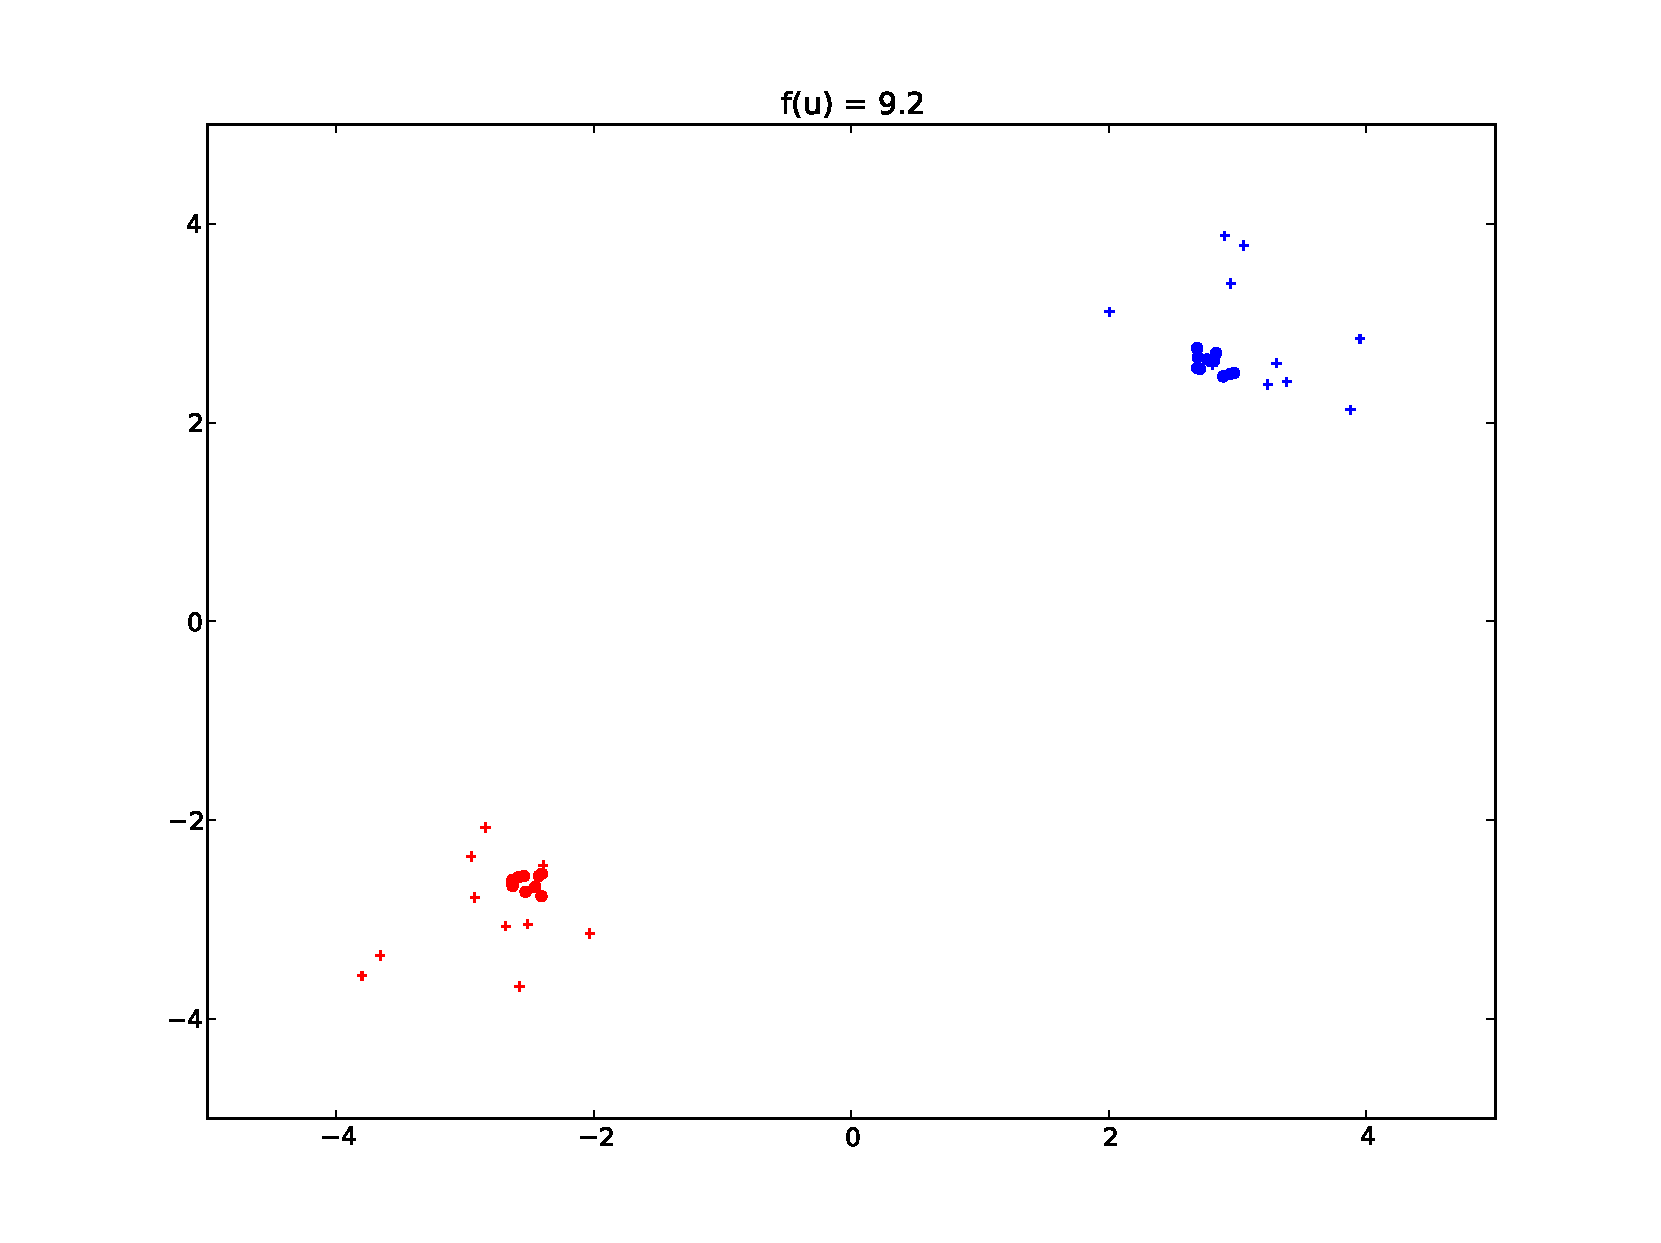
\includegraphics[width=.9\textwidth]{figures/da_w-bin_clust.pdf}
\end{center}
\caption{Clustering utilisant la version non distribuée de l'algorithme.}
\label{fig:da_wbin_clust}
\end{figure}

\begin{figure}
\begin{center}
    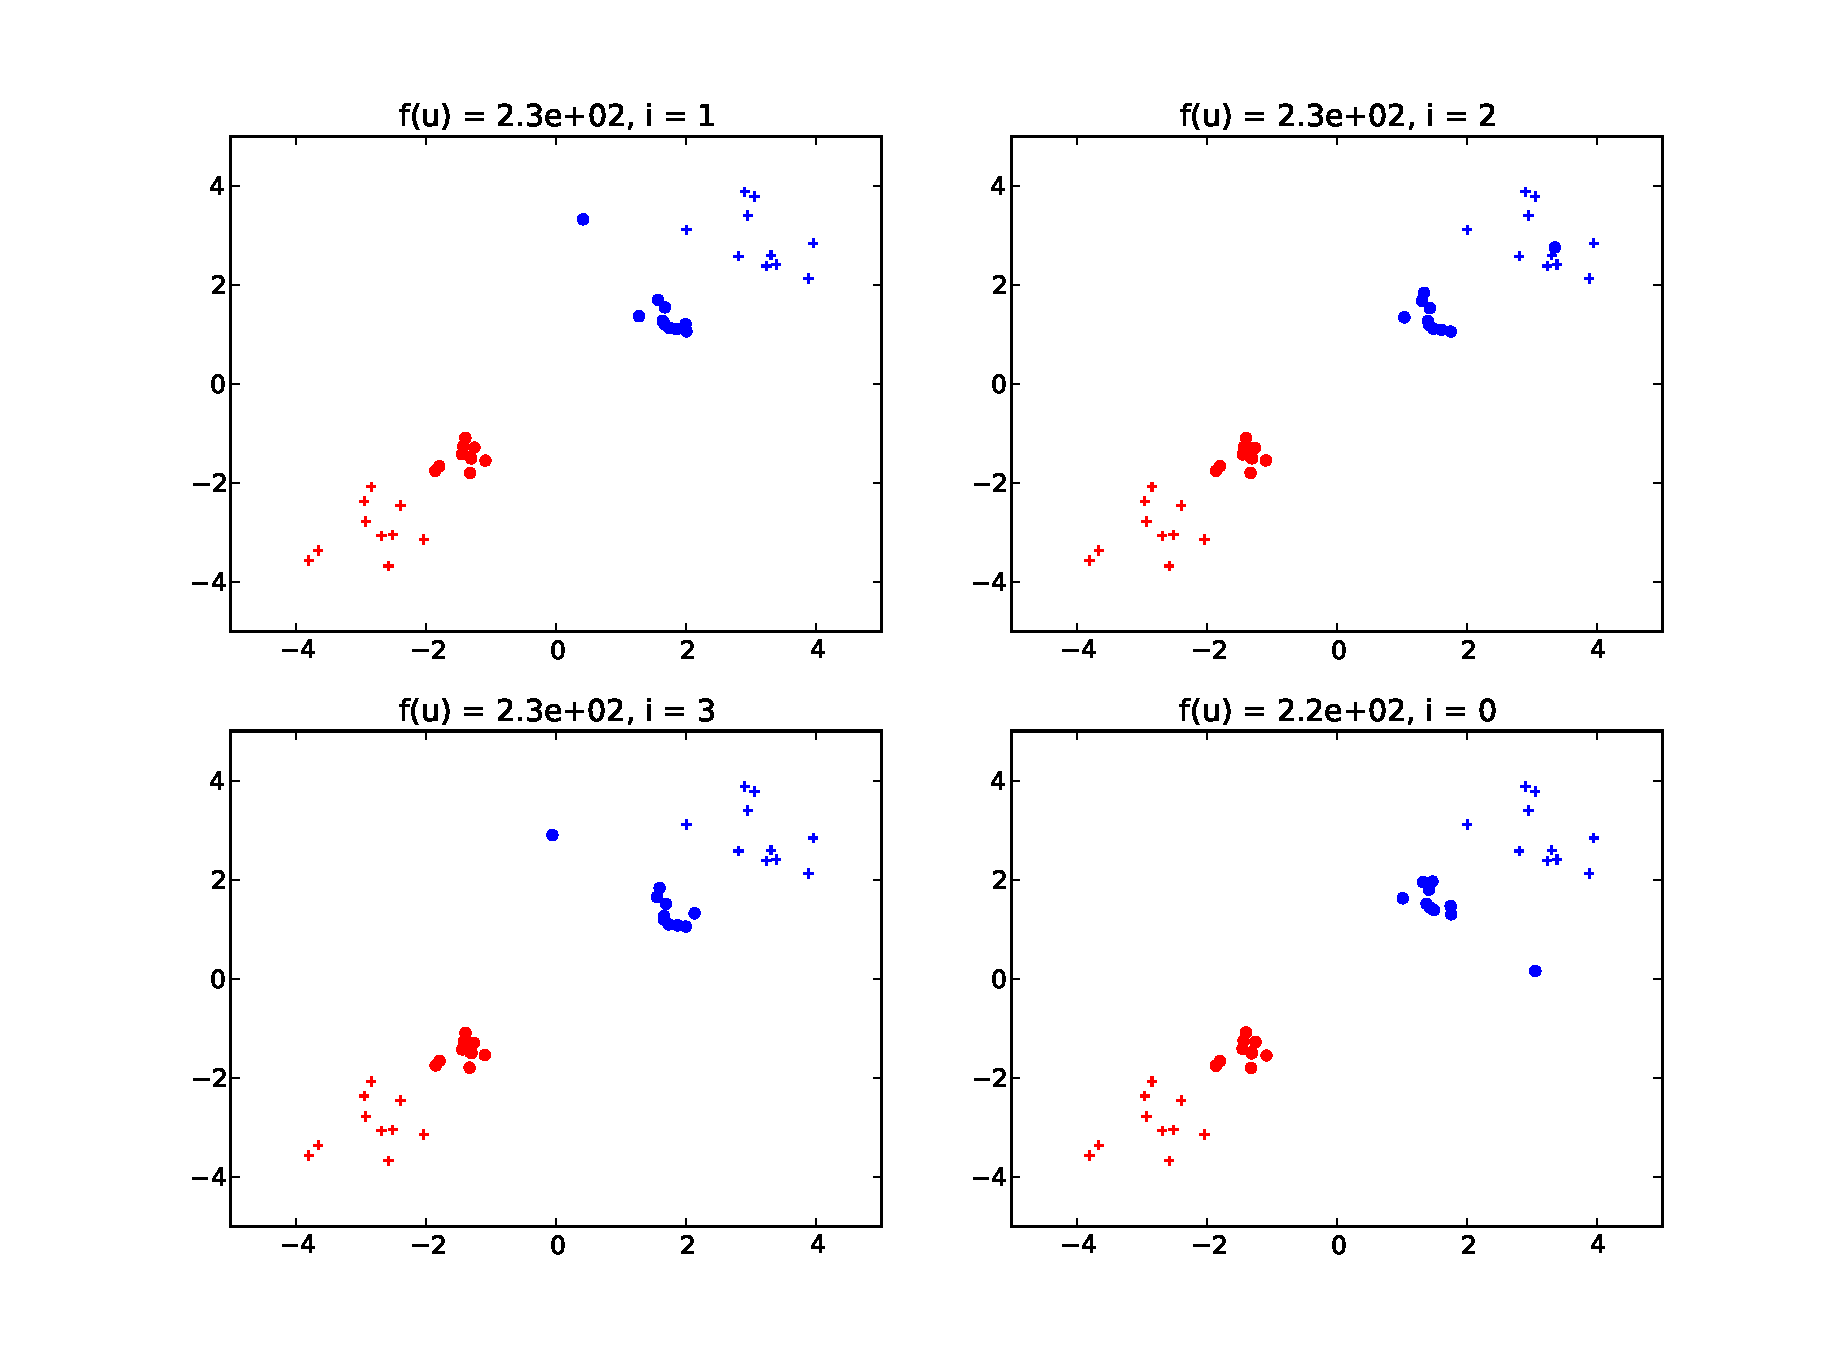
\includegraphics[width=.9\textwidth]{figures/dda_w-bin_clust.pdf}
\end{center}
\caption{Clustering utilisant la version distribuée de l'algorithme}
\label{fig:dda_wbin_clust}
\end{figure}

\begin{figure}
\begin{center}
    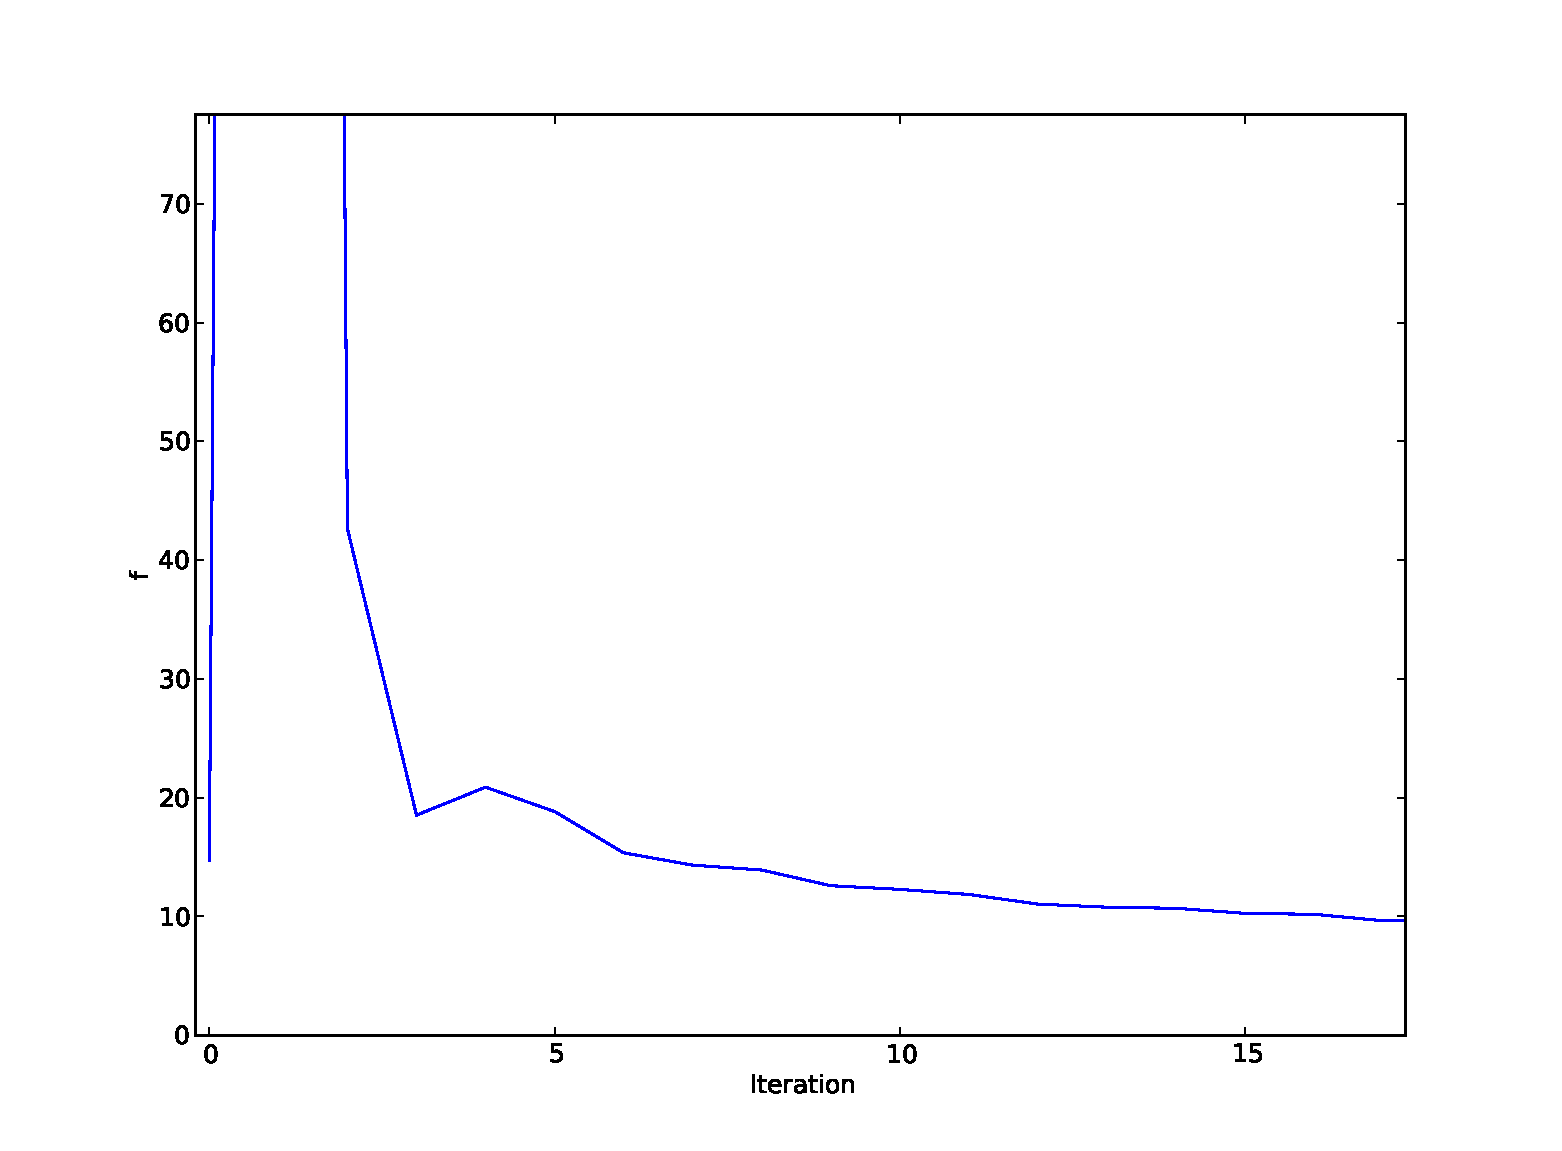
\includegraphics[width=.9\textwidth]{figures/da_w-bin_f.pdf}
\end{center}
\caption{Valeurs de la fonction objectif avec les itérations (version non-distribuée).}
\label{fig:da_wbin_f}
\end{figure}

\begin{figure}
\begin{center}
    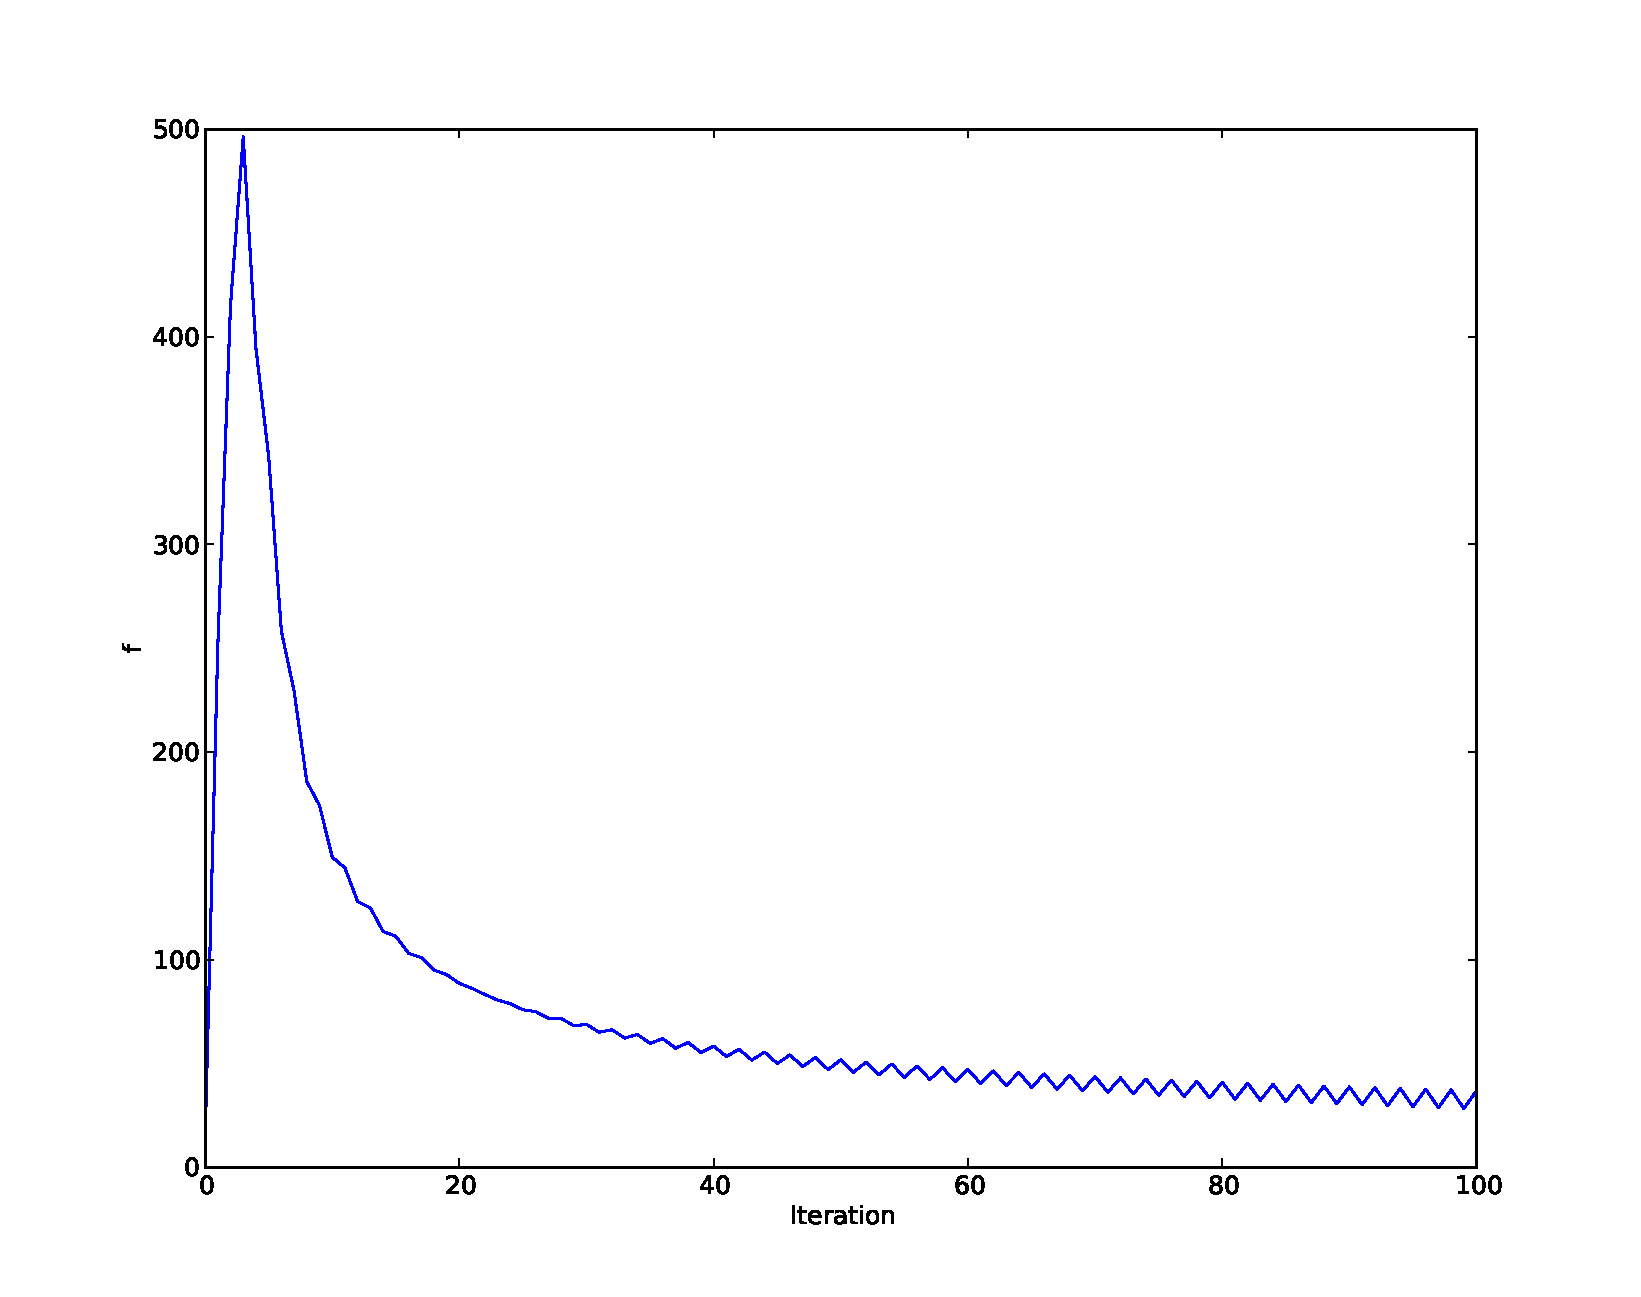
\includegraphics[width=.9\textwidth]{figures/dda_w-bin_f.pdf}
\end{center}
\caption{Valeurs d'une fonction objectif partielle avec les itérations.}
\label{fig:dda_wbin_f}
\end{figure}

\begin{figure}
\begin{center}
    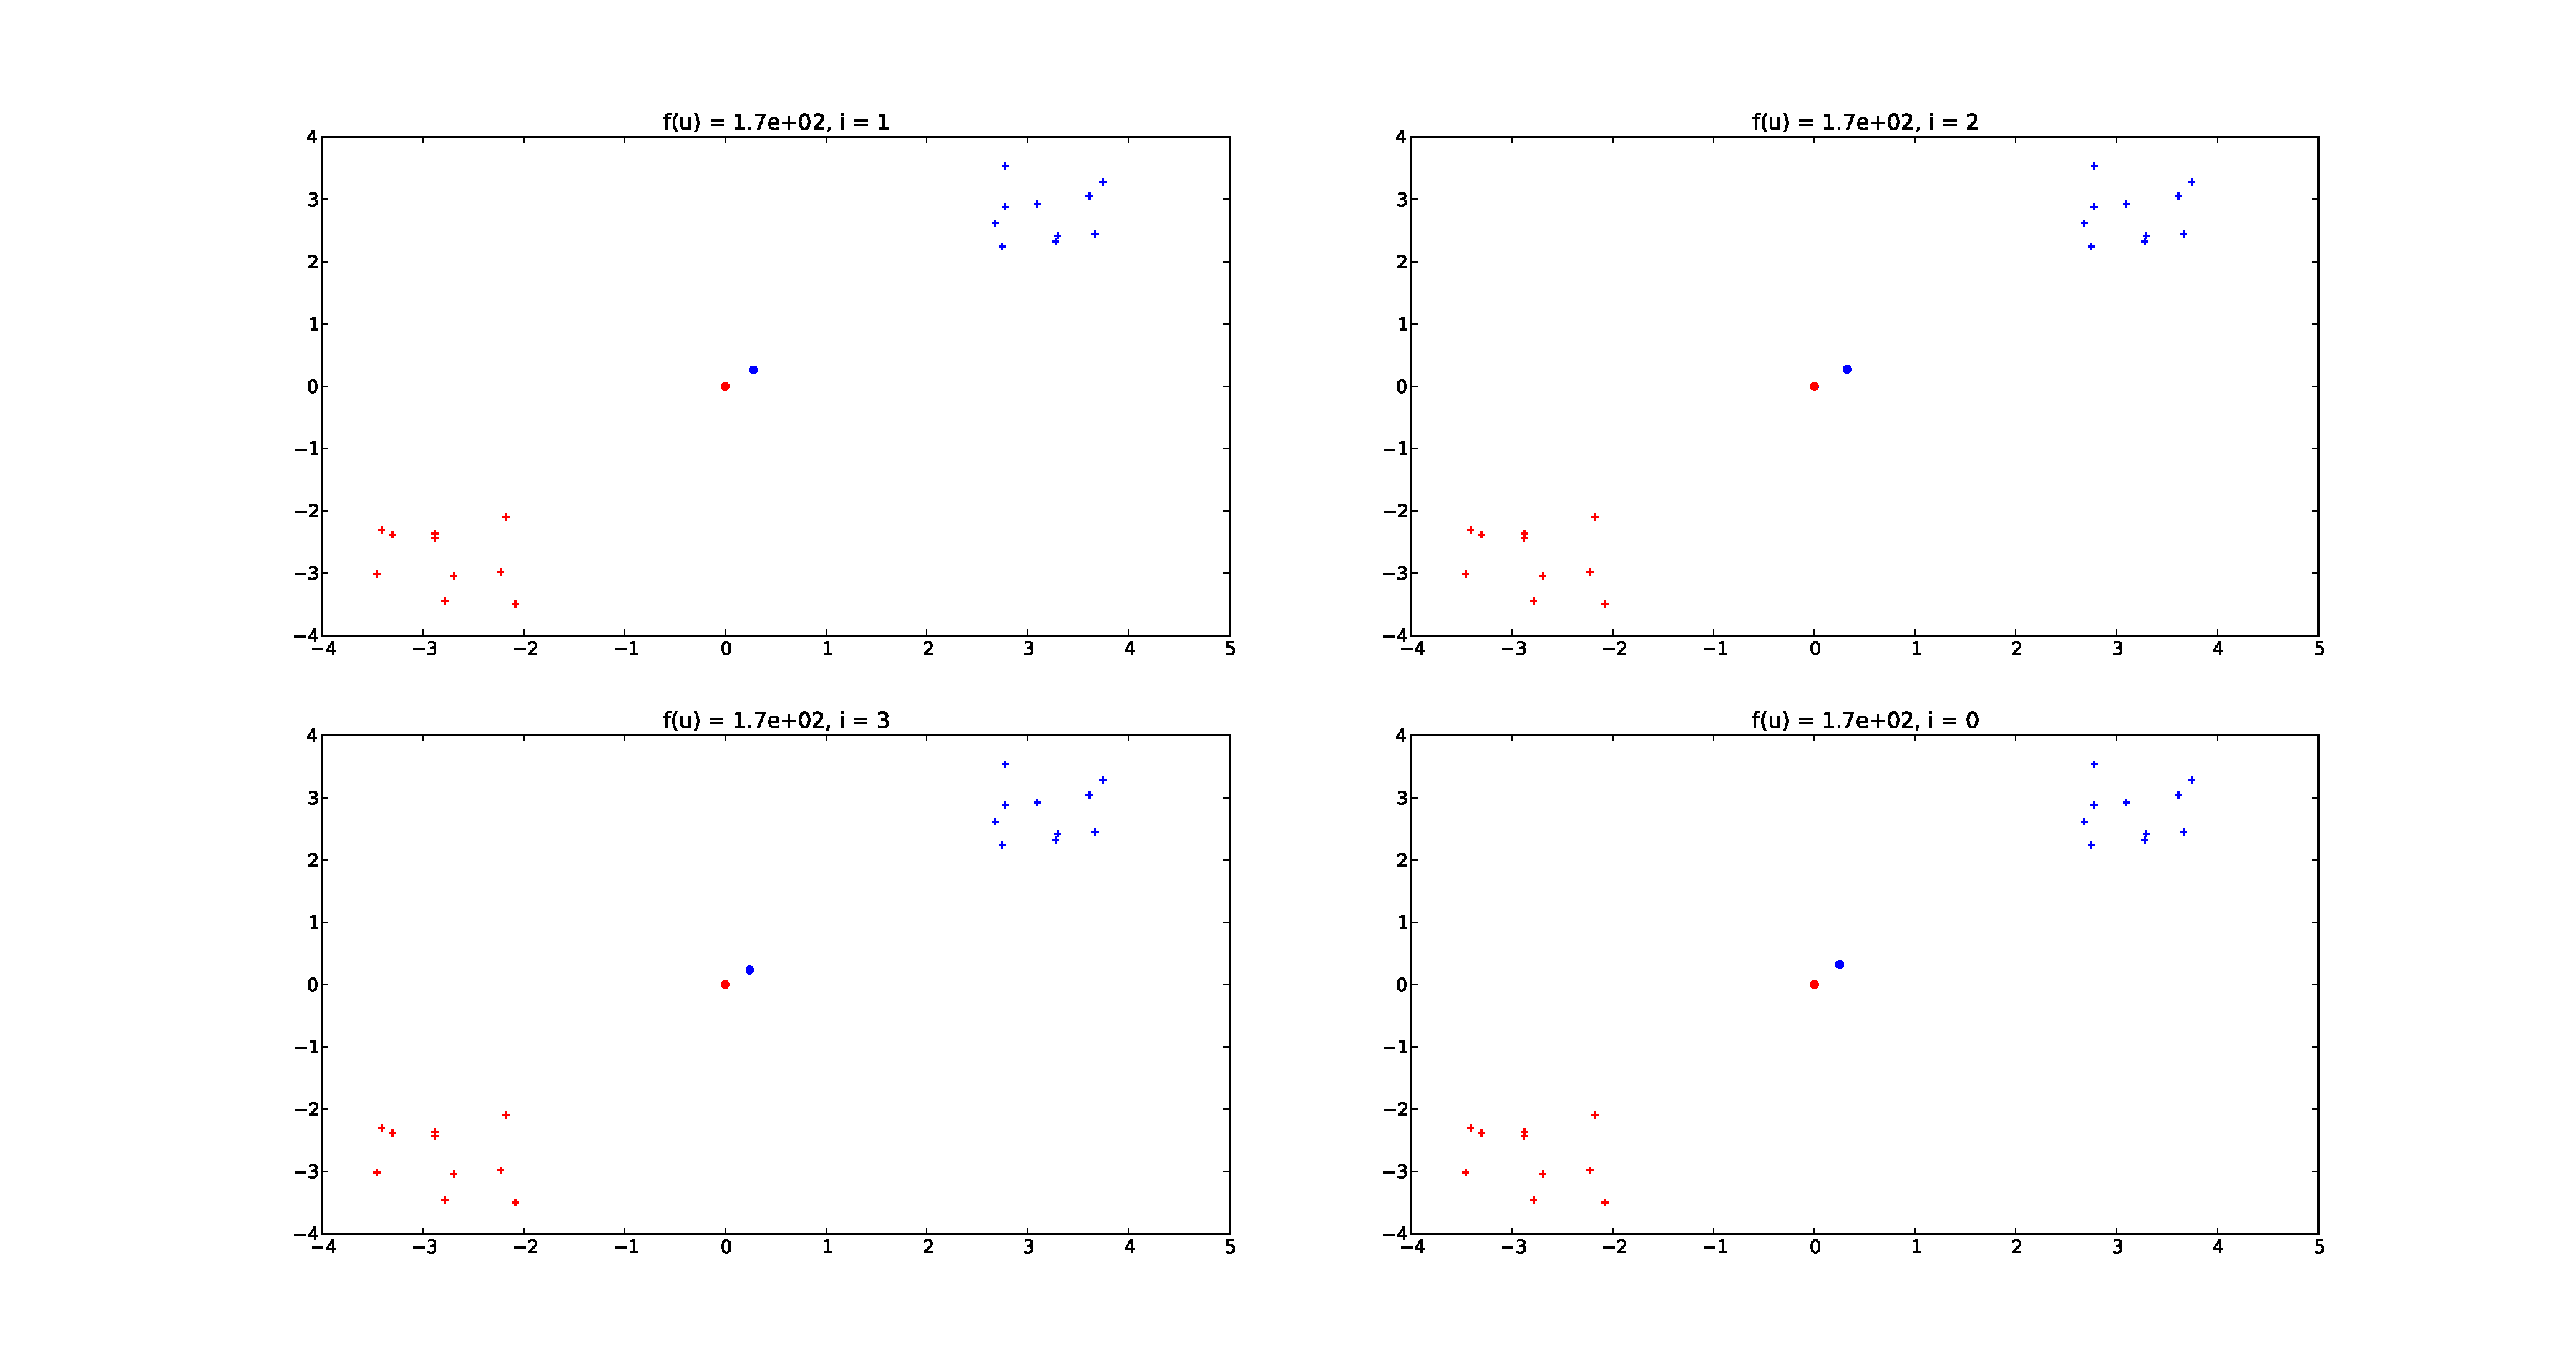
\includegraphics[width=.9\textwidth]{figures/dda_w_clust_G-half.pdf}
\end{center}
\caption{Clustering distribué pour un graphe partiellement connecté (50/50)}
\label{fig:dda_ghalf}
\end{figure}

\begin{figure}
\begin{center}
    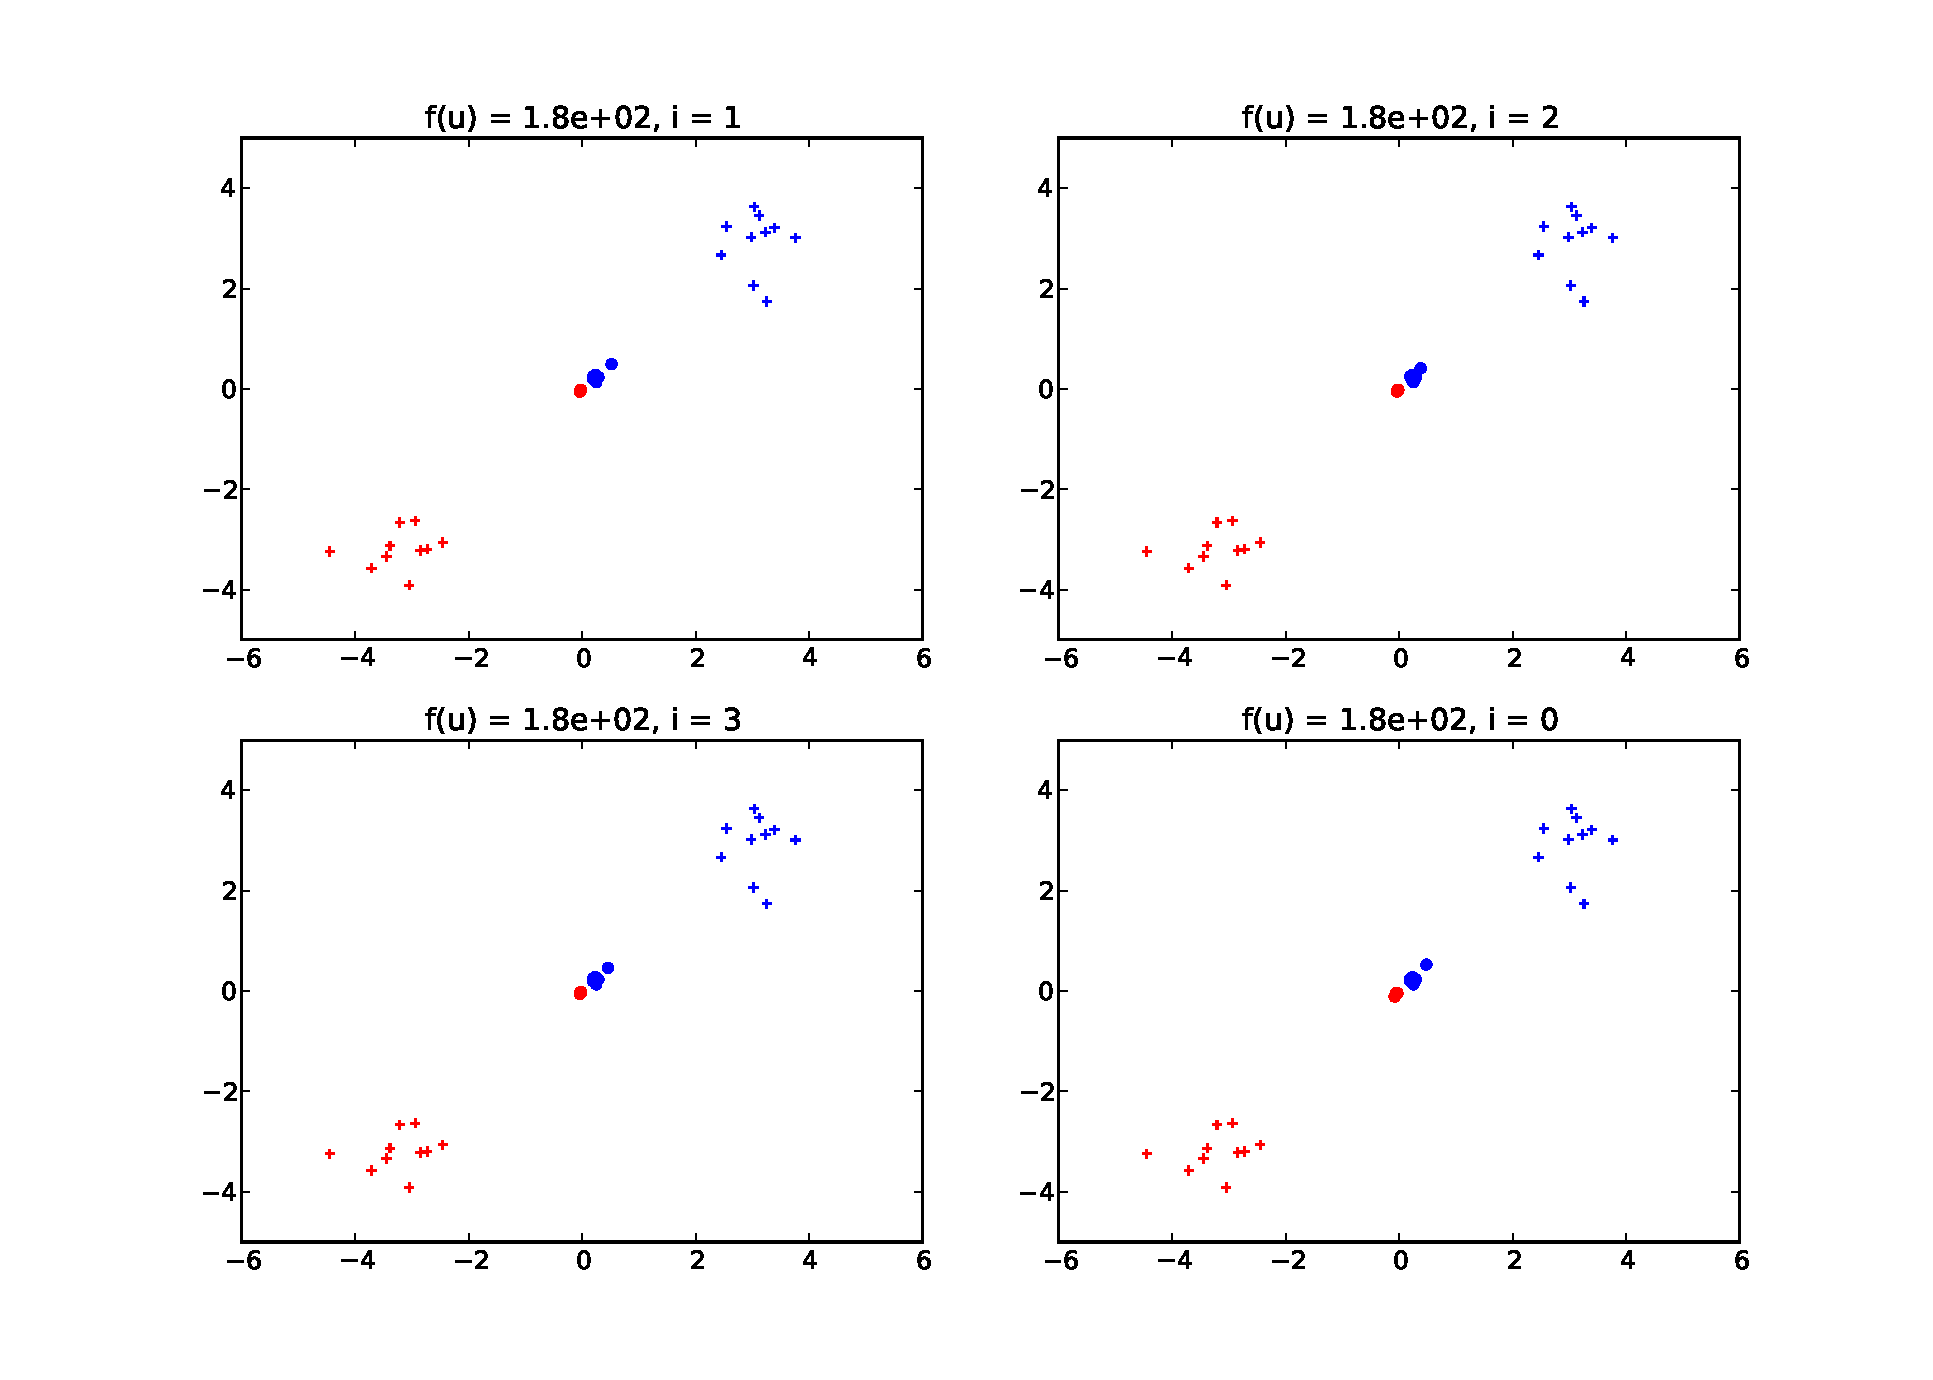
\includegraphics[width=.9\textwidth]{figures/dda_w_clust_G-sep.pdf}
\end{center}
\caption{Clustering distribué pour un graphe partiellement connecté (100/0)}
\label{fig:dda_gsep}
\end{figure}

\end{document}


